\section{Verification} \label{sec:design:verification}
Several of the implementation requirements have been addressed in the chapter \ref{sec:implementation}. In order to verify the implementation and there by design works, 7 tests have been conducted.
\todo{Add what has not been fully implemented}

\todo{Describe in list which requirements are tested.}
\begin{itemize}
	\item \textbf{Session Announcement (Essential metadata)}\\
This test aims to verify the Session Announcement Mechanism with Essential metadata works as intended.
	\item \textbf{Presence Mechanism}\\
This test aims to verify the Presence Mechanism works as intended.
	\item IP collision resolver
This test aims to verify the \pub{} is able to generate a new multicast IP if there is a collision.
	\item Subscribe resolve MG
This test verifies the \sub{} can tage a session name, and resolve that into an multicast IP.
	\item Non-essential Metadata
This test verifies non-essential metadata can be sent and received.
	\item Record with tcpdump and replay with tcpreplay and see subscriber get same data.
This test verifies a stream can be recorded and replayed.
	\item Verify RTCP SR timestamps
This test is supposed to verify RTP SR timestamps are working, however at the moment of writing it does not work.
	\item Compare output from \con{} with output from \program{Snapshot}.
This verifies data sent from snapshot is the same as the \con{} receives.
\end{itemize}


\subsection{Session Announcement \& Essential metadata} \label{sec:verify:sessionannouncement}
This test verifies implementation requirement P8,P9 and S3. The goal of the test is to verify a SDP sent by a \pub{}, and verify a \sub{} can join an announced stream. \todo{add essential metdata tot}
The test has been conducted by staring a \pub{} that streams data from a \con{} which interfaces \program{Snapshot}. In order to verify the SDP is sent as an RTP packet, the traffic sent by the \pub{} has been inspected by \program{tcpdump}. Listing \ref{cmd:verify:sdp} shows the SDP packet sent by the \pub{}.

\begin{listing}[H] 
\begin{minted}{bash}
v=0
o=suas 3736400647 3736400647 IN IP4 batbox3
s=My Session
i=A fun session
u=http://www.ecs.soton.ac.uk/fun/
t=3736400647 3736404247
a=tool:publisher.pl uuid: E9A60146-618C
m=audio 5004 RTP/AVP 96
c=IN IP6 ff15::1234/5
a=quality:5
a=rtpmap:96 L16/220500/1
\end{minted}
\caption{SDP printed by the \pub{}}
\label{lst:verify:sdp}
\end{listing}

Figure \ref{lst:verify:tcpdumpsdp} shows the output from \program{tcpdump}.

\begin{listing}[H] 
	\begin{minted}{bash}
sudo tcpdump -i eth0 -X port 5004
11:04:08.895637 IP6 batbox3.local.5004 > ff15::beef.5004: UDP, length 270
        0x0000:  6006 4601 0116 110a fe80 0000 0000 0000  `.F.............
        0x0010:  ba27 ebff fe5e 2624 ff15 0000 0000 0000  .'...^&\$........
        0x0020:  0000 0000 0000 beef 138c 138c 0116 e83d  ...............=
        0x0030:  8000 0000 0001 e240 23e2 c753 763d 300a  .......@#..Sv=0.
        0x0040:  6f3d 7375 6173 2033 3733 3634 3030 3634  o=suas.373640064
        0x0050:  3720 3337 3336 3430 3036 3437 2049 4e20  7.3736400647.IN.
        0x0060:  4950 3420 6261 7462 6f78 330a 733d 4d79  IP4.batbox3.s=My
        0x0070:  2053 6573 7369 6f6e 0a69 3d41 2066 756e  .Session.i=A.fun
        0x0080:  2073 6573 7369 6f6e 0a75 3d68 7474 703a  .session.u=http:
        0x0090:  2f2f 7777 772e 6563 732e 736f 746f 6e2e  //www.ecs.soton.
        0x00a0:  6163 2e75 6b2f 6675 6e2f 0a74 3d33 3733  ac.uk/fun/.t=373
        0x00b0:  3634 3030 3634 3720 3337 3336 3430 3432  6400647.37364042
        0x00c0:  3437 0a61 3d74 6f6f 6c3a 7075 626c 6973  47.a=tool:publis
        0x00d0:  6865 722e 706c 2075 7569 643a 2045 3941  her.pl.uuid:.E9A
        0x00e0:  3630 3134 362d 3631 3843 0a6d 3d61 7564  60146-618C.m=aud
        0x00f0:  696f 2035 3030 3420 5254 502f 4156 5020  io.5004.RTP/AVP.
        0x0100:  3936 0a63 3d49 4e20 4950 3620 6666 3135  96.c=IN.IP6.ff15
        0x0110:  3a3a 3132 3334 2f35 0a61 3d71 7561 6c69  ::1234/5.a=quali
        0x0120:  7479 3a35 0a61 3d72 7470 6d61 703a 3936  ty:5.a=rtpmap:96
        0x0130:  204c 3136 2f32 3230 3530 302f 310a       .L16/220500/1.
	\end{minted}
\caption{The listing shows the output from \program{tcpdump}, listening on the well known multicast group. The bytes shown before the SDP packet is the ethernet header, UDP header and RTP header}
\label{lst:verify:tcpdumpsdp}
\end{listing}

It should be noted that the ASCII encoded content of the payload corresponds to the SDP packet in listing \ref{lst:verify:sdp}. Furthermore, a session is announce in the key starting with \textbf{C=IN...}.

In listing \ref{lst:verify:subsdp} is the output from a \sub{} shown, that receives the SDP.


\begin{listing}[h] 
\begin{minted}{bash}
SDP from 'publisher.pl uuid: E9A60146-618C', format: audio/L16/220500/1,\
	Multicast: ff15::1234:5004
Joining multicast group: ff15::1234:5004
<SDP printet>
Main-loop stopped with retval: NewRtp
Restarting loop due to new RTP stream joined
\end{minted}
\caption{Listing shows the output from a \sub{} that receives the SDP and joins the stream. It should be noted the event-loop is restarted, in order to also listen for the new multicast group}
\label{lst:verify:subsdp}
\end{listing}



\subsection{Presence Mechanism} \label{sec:verify:presencemechanism}
This test verifies implementation requirement P11-13 and S3. The goal of this test is to verify the presence mechanism works in both \sub{} and \pub{}. Due to lack of time, lists maintaining present participants have not been implemented, however RTCP SDES/BYE are sent and received by both \pub{} and \sub{}.
A test was conducted, where the \pub{} is started and some time later the \sub{} is started. The RTCP SDES sent by the \pub{} and \sub{} is shown in figure \ref{fig:verify:wireshark_presence}.

\begin{figure}[H]
	\centering
	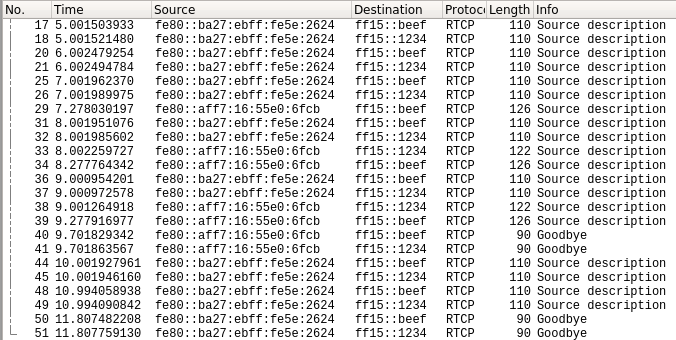
\includegraphics[width=\textwidth]{figures/wireshark_presence}
	\caption{Figure shows output from \program{Wireshark}. It should be noted, that until packet nr.26 is only fe80::ba27:.. sending RTCP SDES, but when \sub{} joins, it starts sending RTCP SDES to both the well known address ff15::beef and the source multicast group ff15::1234.} \label{fig:verify:wireshark_presence}
\end{figure}
From figure \ref{fig:verify:wireshark_presence} the RTCP SDES packets can be seen. Until packet no. 26 is only the \pub{} running. It can be seen that the \pub{} sends its RTCP SDES to both the well known multicast address(ff15::beef) and its source stream (ff15::1234). From packet nr.29, the \sub{} has been started, where it sends out an RTCP SDES to the well known multicast group. It has then joind the source multicast announced by the \pub{} from message no. 32, as the \sub{} sends RTCP SDES to the source stream too. From message no. 40 is the \sub{} gracefully shutting down as it sends a RTCP BYE to both source and well known multicast group. From message no. 50, the \pub{} is gracefully shutting down too.

Listing \ref{lst:verify:rtcpsdes} shows the ouput from a \sub{} receiving and parsing an RTCP SDES packet.

\begin{listing}[h] 
\begin{minted}{bash}
\$VAR1 = bless( {
                 'sdes' => {
                             '6c73c635' => {
                                             'LOC' => '',
                                             'PHONE' => '',
                                             'NAME' => '',
                                             'TOOL' => 'MCLURS',
                                             'NOTE' => '',
                                             'CNAME' => 'suas@batbox3',
                                             'EMAIL' => ''
                                           }
                           }
               }, 'Net::RTCP::Packet' );
\end{minted}
\caption{Listing shows part of the output from a \sub{} receiving and parsing an RTCP SDES packet sent by a \pub{}}
\label{lst:verify:rtcpsdes}
\end{listing}


\subsection{}

\begin{itemize}
	\item Tested with Lua/(post dissector) in wireshark. Transfer chunk of data of 4096 kb(page size) with counter in start of packet. Packet is read from wireshark and by writing dummy producer of 'X' x 4096.

	\item Show Byes are sent when publisher/subscriber are shutdown gracefully

	\item Show essential metadata are sent periodically as json/yml
	\item Show SDES \& BYE to both RTP sessions
	
\end{itemize}
